
\label{chap:experimental_results}


%FIXME: add text here

\subsection{Memory Synchronizer}

This section describes the various tests performed on the full/empty memory synchronizer used within the PDP firmware to synchronize data transitioning across clock domains. First, it discusses simulation results obtained through a full behavioral simulation of PDP. Secondly, it discusses using the memory synchronizer in a test setup and pitfalls that occurred with earlier implementations.

\subsubsection{Simulations}
Figure~\ref{fig:full_empty_sim} shows the simulated results of the full/empty memory synchronizer when transitioning to full and back to empty per clock cycle for a writer and reader operating at \mbox{XXX Mhz} and \mbox{200 Mhz}, respectively. For discussion about each signal and the expected internal behavior see chapter~\ref{sec:memorysync}. Each state transition in the simulation should look similar to the state transitions shown in Table~\ref{tbl:full_empty_circuit_states}.

\begin{figure}
    \centering
    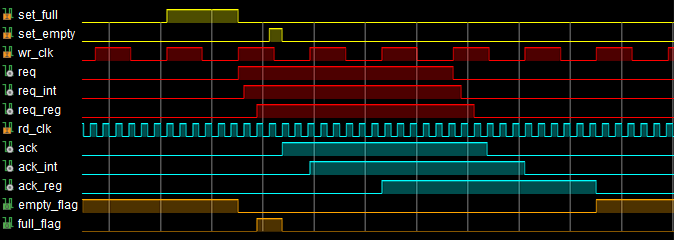
\includegraphics[width=1.0\textwidth]{fig/full_empty_sim.png}
    \caption{Full/Empty Circuit Simulation}
    \label{fig:full_empty_sim}
\end{figure}

The circuit holds a steady state until the {\it set full} signal is toggled for a single {\it write clock} cycle. On the next {\it write clock} cycle, the {\it req signal} transitions high and the {\it empty flag} transitions low. Then the data is moved to the {\it read clock} domain using the two flip-flop synchronizer scheme discussed in the implementation details. At the next rising edge of the {\it read clock}, the data is latched into {\it req internal} which is an internal metastable register. Due to the speed difference between write and read clock speed, the data latches into the register quickly. Following this, a cycle later, the data is clocked into {\it req reg} which completes the {\it read clock} domain transition causes the {\it full flag} to transition high.

Once any corresponding buffer data is handled by the PDP firmware, the {\it set empty} signal is toggled for a single {\it read clock} cycle. This causes the {\it ack} signal to transition high. Then the data is moved to the {\it write clock} domain using the two flip-flop synchronizer scheme discussed in the implementation details. At the next rising edge of the {\it write clock}, the data is latched into {\it ack internal}. Following this, a cycle later, the data is clocked into {\it ack reg} which completes the {\it write clock} domain transition. Notice that it takes much longer to transition data from the {\it read clock} domain to the {\it write clock} domain than vice versa. This is due to the slow write clock.

A {\it write clock} cycle later, {\it req} transitions low. Subsequently, it transitions to the {\it read clock} domain just as before. Following this, the {\it ack} line is lowered and transitions to the {\it write clock} domain just as before. At the same time, the {\it empty flag} transitions high, and the circuit is in the state it began in.

This follows the expected state transitions from Table~\ref{tbl:full_empty_circuit_states} with the only notable distinction being that transitions across clock domains take different amounts of time depending on the destination.

In practice, a complete double handshake takes many cycles to complete which could lead to undesired overflow behavior. In PDP, overflow issues are mitigated by allocating enough internal buffers to allow for there to always be a buffer available for a writer to fill.

Additionally, the use of the two flip-flop synchronizer means that it takes more than a single {\it read clock} cycle for the {\it full flag} to raise; however, given that an IRLED array's pixels take many {\it read clock} cycles to charge, this does not pose a problem. Moreover, in practice, the {\it full flag} will transition in between two to three cycles of the reader clock depending on where the rising edge of the reader clock falls relative to the transitioning of the {\it req} signal.

Figure~\ref{fig:full_empty_row_sim} shows the simulated results of the full/empty memory synchronizer for multiple pixels. The large gaps of time between transitions to full are due to there being multiple buffers available as discussed above. This indicates that at the simulated rates no overflow can occur. In practice, it would be possible for overflow to occur if the write clock speed was close to the read clock speed; however, due to the maximum possible write speed for HDMI only being \mbox{148.5 MHz} and the hiding of clock domain crossinglatency via multiple buffers, a \mbox{200 Mhz} input clock is sufficient for correct behavior.

\begin{figure}
    \centering
    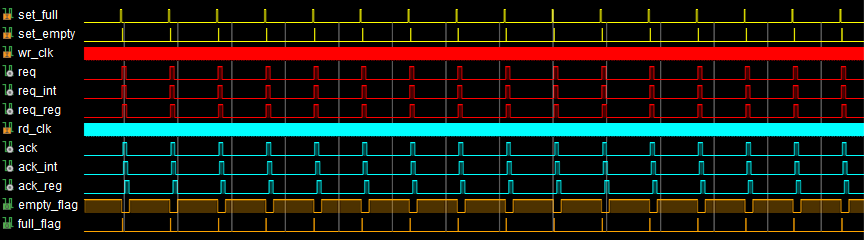
\includegraphics[width=1.0\textwidth]{fig/full_empty_row_sim.png}
    \caption{Full/Empty Circuit Multiple Pixel Simulation}
    \label{fig:full_empty_row_sim}
\end{figure}

\subsubsection{Verification}

\begin{figure}
    \centering
    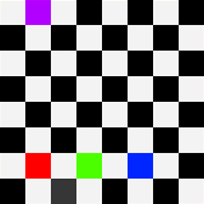
\includegraphics[width=0.25\textwidth]{fig/checker.png}
    \caption{Checker Input Image}
    \label{fig:checker_pattern}
\end{figure}

\begin{figure}
    \centering
    
\includegraphics[width=0.25\textwidth]{fig/random_noise.png}
    \caption{Random Noise Input Image}
    \label{fig:random_noise}
\end{figure}

\subsection{other stuff}
This section provides a few captures of simulation inputs and outputs to show how packets arrive and are processed by the architecture.

In Figure~\ref{fig:input_example} simulated HDMI is shown. When video data enable (write enable) transitions high words of data representing PDP packets start to stream in. These are indicated by Packet ID, X start, X end, Y start, Y end, and Packet Data. Each word would be stored in an SCB slot as indicated in the previous section. The final piece of data indicated is a reset packet. Note, that the data prior to Packet ID would be ignored as it does not represent a valid PDP command. It would be discarded by the valid controller.

\begin{figure}
    \centering
    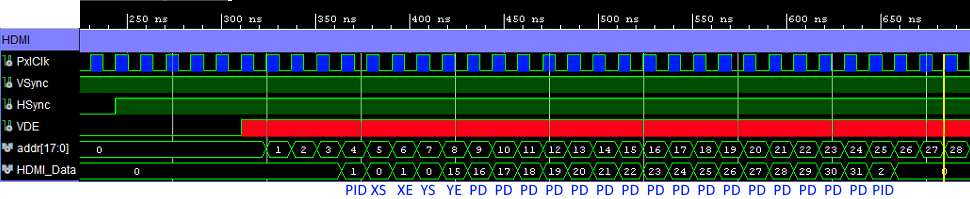
\includegraphics[width=1.0\textwidth]{fig/pdp_input_example.png}
    \caption{PDP Single HDMI Input Example Simulation}
    \label{fig:input_example}
\end{figure}

Figure~\ref{fig:output_example} shows the final output driven to the array. Highlighted in red is data from the write enable packet. Note, all values out are up shifted by 5 bits to be received by the DACs in the system. Additionally, the values are shown in reverse order from the input diagram. For example, 992 corresponds to the value of 31 on the input side. In purple the reset packet is shown with two stages of array writes. In the first stage, load line goes low. In the second stage the load line transitions high.

\begin{figure}
    \centering
    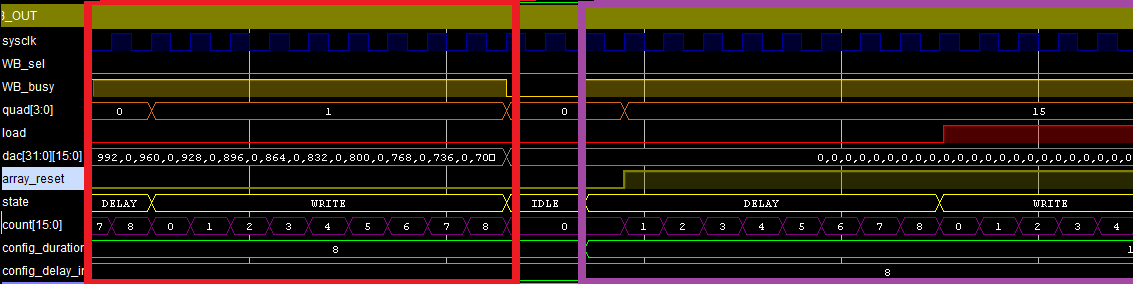
\includegraphics[width=1.0\textwidth]{fig/pdp_output_example.png}
    \caption{PDP Output Example Simulation}
    \label{fig:output_example}
\end{figure}
